% Source Code Guide for Sciara-fv2 CUDA Project
\documentclass[11pt,a4paper]{article}

\usepackage[utf8]{inputenc}
\usepackage[margin=2.5cm]{geometry}
\usepackage{graphicx}
\usepackage{booktabs}
\usepackage{xcolor}
\usepackage{listings}
\usepackage{tikz}
\usetikzlibrary{shapes.geometric, arrows, positioning}
\usepackage{hyperref}
\usepackage{tcolorbox}
\usepackage{enumitem}

% Code listing style
\lstset{
    language=C++,
    basicstyle=\ttfamily\small,
    keywordstyle=\color{blue}\bfseries,
    commentstyle=\color{green!60!black}\itshape,
    stringstyle=\color{red!70!black},
    numbers=left,
    numberstyle=\tiny\color{gray},
    breaklines=true,
    frame=single,
    backgroundcolor=\color{gray!10},
    tabsize=4
}

% Custom boxes for explanations
\newtcolorbox{purposebox}[1][]{
    colback=blue!5,
    colframe=blue!75!black,
    title={\textbf{Muc dich / Purpose}},
    #1
}

\newtcolorbox{keypoint}[1][]{
    colback=yellow!10,
    colframe=orange!75!black,
    title={\textbf{Diem quan trong / Key Point}},
    #1
}

\newtcolorbox{newbie}[1][]{
    colback=green!5,
    colframe=green!50!black,
    title={\textbf{Giai thich cho nguoi moi / Newbie Explanation}},
    #1
}

\title{\Huge\textbf{Huong Dan Source Code}\\[0.5em]
\Large Sciara-fv2 CUDA Lava Flow Simulator\\[1em]
\normalsize Giai thich chi tiet cho nguoi moi bat dau}
\author{Auto-generated Documentation}
\date{\today}

\begin{document}

\maketitle
\tableofcontents
\newpage

%==============================================================================
\section{Tong Quan Project / Project Overview}
%==============================================================================

\subsection{Project nay lam gi? / What does this project do?}

\begin{newbie}
Sciara-fv2 mo phong dong chay cua \textbf{dung nham nui lua} (lava flow).
Tuong tuong ban co mot luoi o vuong (nhu ban co vua), moi o chua thong tin:
\begin{itemize}
    \item \textbf{Sz}: Do cao dia hinh (altitude)
    \item \textbf{Sh}: Do day lava (lava thickness)
    \item \textbf{ST}: Nhiet do lava (temperature)
\end{itemize}
Moi buoc thoi gian, lava chay tu o cao xuong o thap theo trong luc.
\end{newbie}

\subsection{Cau truc thu muc / Directory Structure}

\begin{verbatim}
draft_sciara-fv2/
|-- Sciara.cu              <- Quan ly bo nho GPU (Unified Memory)
|-- sciara_fv2.cu          <- Version 1: Global Memory (baseline)
|-- sciara_fv2_tiled.cu    <- Version 2: Shared Memory (no halo)
|-- sciara_fv2_tiled_halo.cu <- Version 3: Shared Memory (with halo)
|-- sciara_fv2_cfame.cu    <- Version 4: Atomic operations (giu Mf)
|-- sciara_fv2_cfamo.cu    <- Version 5: Atomic (bo Mf) - NHANH NHAT
|-- block_size_exploration.cu <- Tool test cac kich thuoc block
|-- Sciara.h, io.cpp, ...  <- Header va file ho tro
\end{verbatim}

%==============================================================================
\section{So Do Phat Trien / Evolution Diagram}
%==============================================================================

\begin{center}
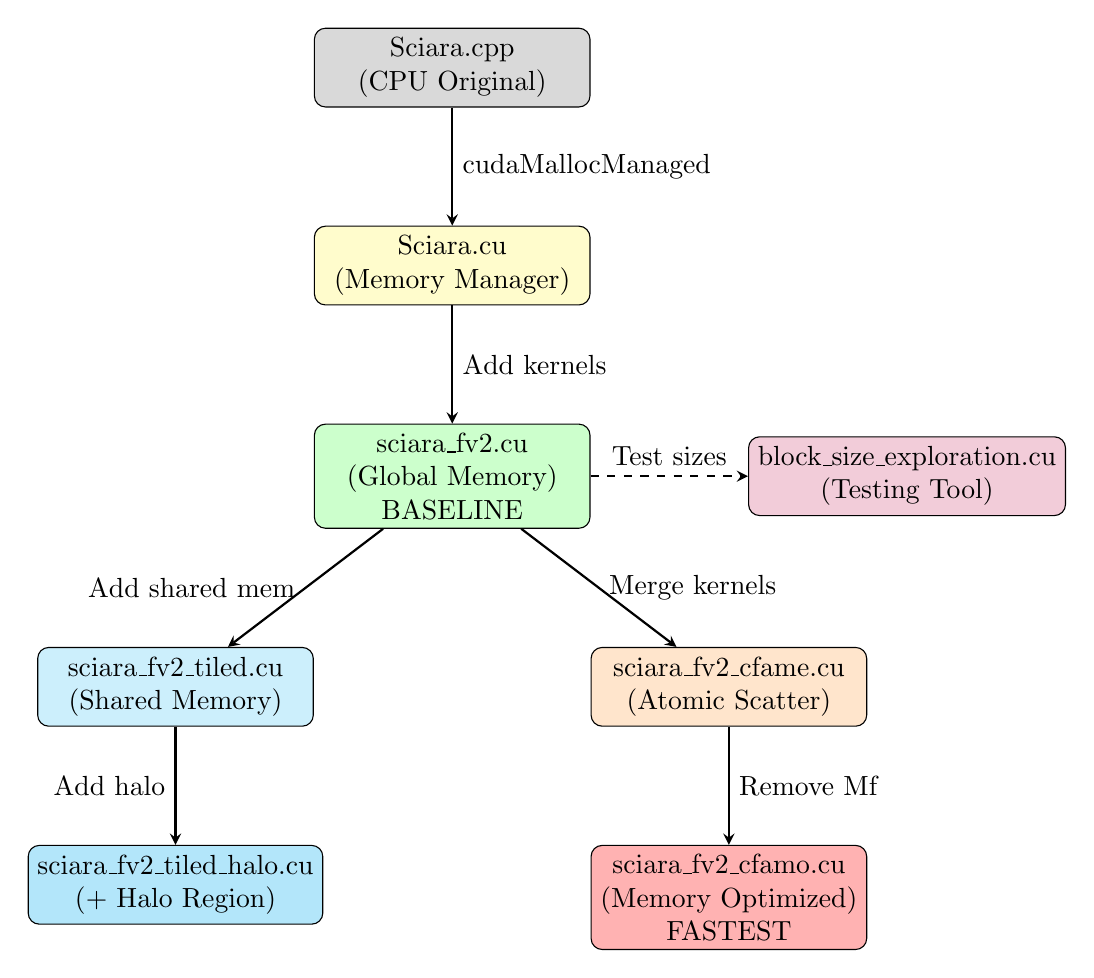
\begin{tikzpicture}[
    node distance=1.5cm,
    box/.style={rectangle, draw, rounded corners, minimum width=3.5cm, minimum height=1cm, align=center, fill=blue!10},
    arrow/.style={->, thick, >=stealth}
]

% Original file
\node[box, fill=gray!30] (original) {Sciara.cpp\\(CPU Original)};

% Sciara.cu
\node[box, below=of original, fill=yellow!20] (sciaracu) {Sciara.cu\\(Memory Manager)};

% Global version
\node[box, below=of sciaracu, fill=green!20] (global) {sciara\_fv2.cu\\(Global Memory)\\BASELINE};

% Tiled versions
\node[box, below left=1.5cm and 0cm of global, fill=cyan!20] (tiled) {sciara\_fv2\_tiled.cu\\(Shared Memory)};

\node[box, below=of tiled, fill=cyan!30] (halo) {sciara\_fv2\_tiled\_halo.cu\\(+ Halo Region)};

% Atomic versions
\node[box, below right=1.5cm and 0cm of global, fill=orange!20] (cfame) {sciara\_fv2\_cfame.cu\\(Atomic Scatter)};

\node[box, below=of cfame, fill=red!30] (cfamo) {sciara\_fv2\_cfamo.cu\\(Memory Optimized)\\FASTEST};

% Tool
\node[box, right=2cm of global, fill=purple!20] (explore) {block\_size\_exploration.cu\\(Testing Tool)};

% Arrows
\draw[arrow] (original) -- (sciaracu) node[midway, right] {cudaMallocManaged};
\draw[arrow] (sciaracu) -- (global) node[midway, right] {Add kernels};
\draw[arrow] (global) -- (tiled) node[midway, left] {Add shared mem};
\draw[arrow] (tiled) -- (halo) node[midway, left] {Add halo};
\draw[arrow] (global) -- (cfame) node[midway, right] {Merge kernels};
\draw[arrow] (cfame) -- (cfamo) node[midway, right] {Remove Mf};
\draw[arrow, dashed] (global) -- (explore) node[midway, above] {Test sizes};

\end{tikzpicture}
\end{center}

%==============================================================================
\section{Sciara.cu - Bo Nho GPU / GPU Memory Manager}
%==============================================================================

\begin{purposebox}
File nay thay the \texttt{Sciara.cpp} (CPU) de cap phat bo nho tren GPU.
Su dung \textbf{CUDA Unified Memory} de CPU va GPU dung chung bo nho.
\end{purposebox}

\subsection{Ham allocateSubstates() - Cap phat bo nho}

\begin{lstlisting}[caption={Cap phat bo nho Unified Memory}]
void allocateSubstates(Sciara *sciara)
{
    int size = sciara->domain->rows * sciara->domain->cols;

    // cudaMallocManaged: Cap phat bo nho dung chung CPU-GPU
    CUDA_CHECK(cudaMallocManaged(&sciara->substates->Sz,
               sizeof(double) * size));
    // Sz_next, Sh, Sh_next, ST, ST_next, Mf, Mb, Mhs tuong tu...
}
\end{lstlisting}

\begin{newbie}
\textbf{cudaMallocManaged} khac \texttt{malloc} o cho:
\begin{itemize}
    \item \texttt{malloc}: Chi CPU doc/ghi duoc
    \item \texttt{cudaMalloc}: Chi GPU doc/ghi duoc
    \item \texttt{cudaMallocManaged}: CA HAI CPU va GPU deu doc/ghi duoc!
\end{itemize}
Khi GPU can du lieu, no tu dong copy tu CPU sang. Rat tien loi!
\end{newbie}

\subsection{Cac mang du lieu chinh / Main Data Arrays}

\begin{table}[h]
\centering
\caption{Cac mang substate va y nghia}
\begin{tabular}{@{}llp{7cm}@{}}
\toprule
\textbf{Mang} & \textbf{Kieu} & \textbf{Y nghia} \\
\midrule
Sz, Sz\_next & double[] & Do cao dia hinh (altitude). \texttt{\_next} la gia tri sau buoc tiep theo. \\
Sh, Sh\_next & double[] & Do day lava. Thay doi khi lava chay. \\
ST, ST\_next & double[] & Nhiet do lava. Giam dan theo thoi gian. \\
Mf & double[] & Flow buffer: Luu luong lava chay giua cac o (8 huong x cells). \\
Mb & bool[] & Boundary mask: Danh dau o bien. \\
Mhs & double[] & Solidified height: Lava da dong dac. \\
\bottomrule
\end{tabular}
\end{table}

%==============================================================================
\section{sciara\_fv2.cu - Version Global Memory (Baseline)}
%==============================================================================

\begin{purposebox}
Day la version \textbf{co ban nhat}. Tat ca kernel doc/ghi truc tiep tu \textbf{Global Memory} (bo nho chinh cua GPU). Dung lam baseline de so sanh voi cac version toi uu.
\end{purposebox}

\subsection{Cau truc kernel chay moi buoc / Kernel Execution Order}

\begin{center}
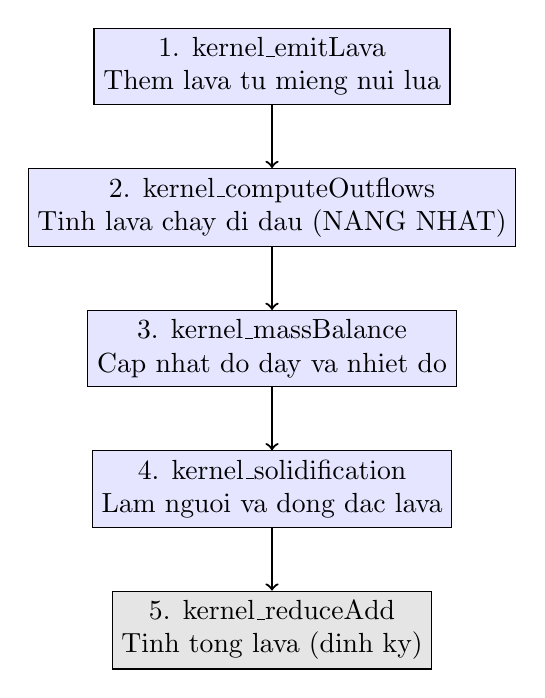
\begin{tikzpicture}[
    node distance=0.8cm,
    box/.style={rectangle, draw, minimum width=4cm, minimum height=0.8cm, align=center, fill=blue!10}
]
\node[box] (emit) {1. kernel\_emitLava\\Them lava tu mieng nui lua};
\node[box, below=of emit] (outflow) {2. kernel\_computeOutflows\\Tinh lava chay di dau (NANG NHAT)};
\node[box, below=of outflow] (mass) {3. kernel\_massBalance\\Cap nhat do day va nhiet do};
\node[box, below=of mass] (solid) {4. kernel\_solidification\\Lam nguoi va dong dac lava};
\node[box, below=of solid, fill=gray!20] (reduce) {5. kernel\_reduceAdd\\Tinh tong lava (dinh ky)};

\draw[->, thick] (emit) -- (outflow);
\draw[->, thick] (outflow) -- (mass);
\draw[->, thick] (mass) -- (solid);
\draw[->, thick] (solid) -- (reduce);
\end{tikzpicture}
\end{center}

\subsection{kernel\_computeOutflows - Kernel nang nhat}

\begin{lstlisting}[caption={Kernel tinh huong chay cua lava}]
__global__ void kernel_computeOutflows(
    int r, int c,           // Kich thuoc luoi
    double* Sz, double* Sh, double* ST, double* Mf,  // Du lieu
    double Pc, double _a, double _b, double _c, double _d)  // Tham so
{
    // Tinh vi tri cell hien tai tu thread ID
    int j = blockIdx.x * blockDim.x + threadIdx.x;
    int i = blockIdx.y * blockDim.y + threadIdx.y;

    if (i >= r || j >= c) return;  // Kiem tra bien

    double h0 = GET(Sh, c, i, j);  // Lay do day lava cell nay
    if (h0 <= 0) return;           // Khong co lava -> khong lam gi

    // Vong lap qua 8 o lan can (Moore neighborhood)
    for (int k = 0; k < MOORE_NEIGHBORS; k++) {
        int ni = i + d_Xi[k];  // Toa do o lan can
        int nj = j + d_Xj[k];
        // ... tinh flow dua tren gradient do cao ...
    }

    // Luu flow vao Mf buffer
    BUF_SET(Mf, r, c, k-1, i, j, flow);
}
\end{lstlisting}

\begin{newbie}
\textbf{Moore Neighborhood} la 8 o xung quanh mot o:
\begin{verbatim}
    [5]  [1]  [6]
    [2]  [0]  [3]     <- [0] la cell hien tai
    [7]  [4]  [8]
\end{verbatim}
Moi cell tinh xem lava se chay sang o nao (dua vao do cao + do day lava).
\end{newbie}

\subsection{Tai sao Global Memory cham?}

\begin{keypoint}
Moi lan doc \texttt{GET(Sh, c, ni, nj)} phai di qua Global Memory (cham ~400 cycles).
Kernel \texttt{computeOutflows} doc 9 o (1 center + 8 neighbors) cho MOI cell.\\
$\Rightarrow$ Rat nhieu lan truy cap bo nho!
\end{keypoint}

%==============================================================================
\section{sciara\_fv2\_tiled.cu - Shared Memory (Khong Halo)}
%==============================================================================

\begin{purposebox}
Toi uu bang cach load du lieu vao \textbf{Shared Memory} (bo nho nhanh tren chip).
Moi block load 1 tile (16x16) vao shared memory truoc khi tinh toan.
\end{purposebox}

\subsection{Y tuong Tiling}

\begin{center}
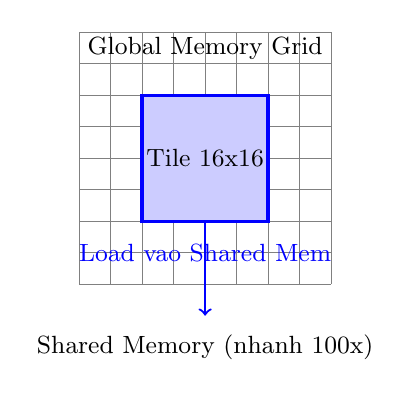
\begin{tikzpicture}[scale=0.4]
% Grid
\draw[step=1, gray, thin] (0,0) grid (8,8);
% Tile highlight
\fill[blue!20] (2,2) rectangle (6,6);
\draw[blue, very thick] (2,2) rectangle (6,6);
% Labels
\node at (4, 4) {\small Tile 16x16};
\node at (4, 7.5) {\small Global Memory Grid};
\node[blue] at (4, 1) {\small Load vao Shared Mem};

% Arrow to shared memory
\draw[->, thick, blue] (4, 2) -- (4, -1);
\node at (4, -2) {\small Shared Memory (nhanh 100x)};
\end{tikzpicture}
\end{center}

\subsection{Code Load Tile vao Shared Memory}

\begin{lstlisting}[caption={Load tile vao shared memory}]
__shared__ double s_Sz[TILE_SIZE_Y][TILE_SIZE_X];  // 16x16 = 2KB
__shared__ double s_Sh[TILE_SIZE_Y][TILE_SIZE_X];
__shared__ double s_ST[TILE_SIZE_Y][TILE_SIZE_X];

// Moi thread load 1 element
if (i < r && j < c) {
    s_Sz[ty][tx] = GET(Sz, c, i, j);  // Doc tu global
    s_Sh[ty][tx] = GET(Sh, c, i, j);
    s_ST[ty][tx] = GET(ST, c, i, j);
}
__syncthreads();  // Doi tat ca thread load xong

// Gio dung s_Sz, s_Sh, s_ST thay vi doc global!
\end{lstlisting}

\begin{keypoint}
\textbf{Van de}: Thread o bien tile (25\%) van phai doc neighbor tu global memory vi neighbor nam ngoai tile. Day la ly do can \textbf{Halo version}.
\end{keypoint}

%==============================================================================
\section{sciara\_fv2\_tiled\_halo.cu - Shared Memory (Co Halo)}
%==============================================================================

\begin{purposebox}
Giai quyet van de border bang cach load them 1 lop o bao quanh tile (\textbf{halo}).
Tile 16x16 tro thanh 18x18 trong shared memory.
\end{purposebox}

\subsection{Halo Region Visualization}

\begin{center}
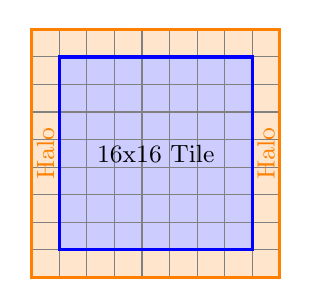
\begin{tikzpicture}[scale=0.35]
% Outer (halo)
\fill[orange!20] (0,0) rectangle (9,9);
% Inner (tile)
\fill[blue!20] (1,1) rectangle (8,8);

\draw[step=1, gray] (0,0) grid (9,9);
\draw[blue, very thick] (1,1) rectangle (8,8);
\draw[orange, very thick] (0,0) rectangle (9,9);

\node at (4.5, 4.5) {\small 16x16 Tile};
\node[orange] at (0.5, 4.5) {\rotatebox{90}{\small Halo}};
\node[orange] at (8.5, 4.5) {\rotatebox{90}{\small Halo}};
\end{tikzpicture}
\end{center}

\begin{lstlisting}[caption={Shared memory voi halo}]
#define TILE_SIZE 16
#define HALO_SIZE 1
#define BLOCK_SIZE (TILE_SIZE + 2*HALO_SIZE)  // 18

__shared__ double s_Sz[BLOCK_SIZE][BLOCK_SIZE];  // 18x18 = 2.6KB
\end{lstlisting}

\begin{newbie}
\textbf{Tai sao Halo?} Khi tinh cell (1,1) trong tile, can doc cell (0,0) la neighbor.
Neu khong co halo, (0,0) nam ngoai tile $\Rightarrow$ phai doc global (cham).
Voi halo, (0,0) da duoc load vao shared memory $\Rightarrow$ doc nhanh!
\end{newbie}

\subsection{Tai sao Tiled versions van cham hon Global?}

\begin{keypoint}
Cho grid nho nhu 517x378:
\begin{enumerate}
    \item \texttt{\_\_syncthreads()} ton ~50 cycles moi lan
    \item L2 Cache (2MB) cua GTX 980 da du lon cache toan bo data
    \item Overhead load halo khong bu dap duoc loi ich
\end{enumerate}
$\Rightarrow$ Tiled chi tot khi grid > 2048x2048 (vuot qua L2 cache).
\end{keypoint}

%==============================================================================
\section{sciara\_fv2\_cfame.cu - Atomic Scatter Pattern}
%==============================================================================

\begin{purposebox}
Thay doi tu \textbf{Gather} (doc tu neighbors) sang \textbf{Scatter} (ghi den neighbors).
Gop \texttt{computeOutflows} va \texttt{massBalance} thanh 1 kernel, dung \textbf{atomic operations}.
\end{purposebox}

\subsection{Gather vs Scatter}

\begin{center}
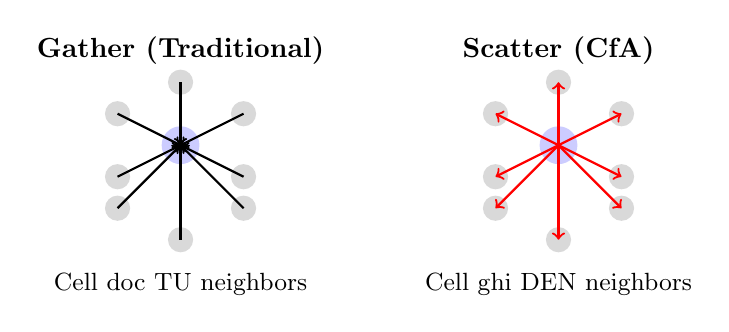
\begin{tikzpicture}[scale=0.8]
% Gather
\begin{scope}
\node at (2, 3) {\textbf{Gather (Traditional)}};
\fill[blue!20] (2,1.5) circle (0.3);
\foreach \x/\y in {1/2, 2/2.5, 3/2, 1/1, 3/1, 1/0.5, 2/0, 3/0.5} {
    \fill[gray!30] (\x, \y) circle (0.2);
    \draw[->, thick] (\x, \y) -- (2, 1.5);
}
\node at (2, -0.7) {\small Cell doc TU neighbors};
\end{scope}

% Scatter
\begin{scope}[xshift=6cm]
\node at (2, 3) {\textbf{Scatter (CfA)}};
\fill[blue!20] (2,1.5) circle (0.3);
\foreach \x/\y in {1/2, 2/2.5, 3/2, 1/1, 3/1, 1/0.5, 2/0, 3/0.5} {
    \fill[gray!30] (\x, \y) circle (0.2);
    \draw[->, thick, red] (2, 1.5) -- (\x, \y);
}
\node at (2, -0.7) {\small Cell ghi DEN neighbors};
\end{scope}
\end{tikzpicture}
\end{center}

\subsection{Tai sao can Atomic?}

\begin{lstlisting}[caption={Van de race condition}]
// Cell A ghi vao cell X: Sh_next[X] += flowA
// Cell B CUNG ghi vao cell X: Sh_next[X] += flowB
// Neu chay song song -> mat du lieu!

// Giai phap: Dung atomic
atomicAddDouble(&Sh_next[ni * c + nj], flow);  // Dam bao khong mat
\end{lstlisting}

\begin{newbie}
\textbf{atomicAdd} dam bao rang khi nhieu thread ghi vao cung mot o nho,
tat ca gia tri deu duoc cong dung. Khong co atomic, chi 1 gia tri duoc luu!
\end{newbie}

\subsection{Temperature Accumulation Trick}

\begin{lstlisting}[caption={Trick tinh nhiet do trung binh}]
// Van de: Khong the atomic tinh trung binh!
// T_avg = (h1*T1 + h2*T2) / (h1+h2)

// Giai phap: Luu h*T thay vi T
SET(ST_next, c, i, j, sh * st);  // Luu tich h*T

// Sau khi xong tat ca atomic add:
kernel_normalizeTemperature<<<...>>>();
// T = ST_next / Sh_next  (lay lai nhiet do)
\end{lstlisting}

%==============================================================================
\section{sciara\_fv2\_cfamo.cu - Memory Optimized (NHANH NHAT)}
%==============================================================================

\begin{purposebox}
Toi uu them tu CfAMe bang cach \textbf{bo mang Mf} (12.5MB).
Flow duoc tinh va dung ngay, khong luu trung gian.
\end{purposebox}

\subsection{Khac biet voi CfAMe}

\begin{table}[h]
\centering
\begin{tabular}{@{}lcc@{}}
\toprule
& \textbf{CfAMe} & \textbf{CfAMo} \\
\midrule
Mf buffer & Co (12.5 MB) & Khong (0 MB) \\
Debug flow values & Duoc & Khong \\
Memory bandwidth & Cao hon & Thap hon \\
Speedup vs Global & 1.10x & \textbf{1.16x} \\
\bottomrule
\end{tabular}
\end{table}

\begin{lstlisting}[caption={CfAMo khong luu Mf}]
// CfAMe: Luu flow vao Mf
BUF_SET(Mf, r, c, k-1, i, j, flow);  // <- BO DONG NAY
atomicAddDouble(&Sh_next[...], flow);

// CfAMo: Dung flow truc tiep
if (flow > 0) {
    atomicAddDouble(&Sh_next[ni * c + nj], flow);
    // Khong luu Mf -> tiet kiem bo nho
}
\end{lstlisting}

\subsection{Tai sao CfAMo nhanh nhat?}

\begin{keypoint}
\begin{enumerate}
    \item \textbf{It kernel launches}: 3 thay vi 4 (tiet kiem overhead)
    \item \textbf{It memory}: Khong co Mf 12.5MB $\Rightarrow$ cache hit tot hon
    \item \textbf{Atomic contention thap}: Chi ~30\% cells co lava active
\end{enumerate}
\end{keypoint}

%==============================================================================
\section{block\_size\_exploration.cu - Tool Benchmark}
%==============================================================================

\begin{purposebox}
Chuong trinh nho de test cac kich thuoc block khac nhau (8x8, 16x16, 32x32, v.v.)
va do thoi gian chay, occupancy.
\end{purposebox}

\begin{lstlisting}[caption={Chay tool}]
$ make block_explore
$ ./block_explore

| Block | Thrds | Grid Size | Neighbor | Elemwise | Occupancy |
|-------|-------|-----------|----------|----------|-----------|
| 8x8   |  64   | (65, 48)  |   0.125  |   0.042  |   50.0%   |
|16x16  | 256   | (33, 24)  |   0.098  |   0.038  |  100.0%   |  <- Tot
|32x32  |1024   | (17, 12)  |   0.112  |   0.041  |   50.0%   |
\end{lstlisting}

%==============================================================================
\section{Tong Ket / Summary}
%==============================================================================

\begin{table}[h]
\centering
\caption{So sanh 5 CUDA versions}
\begin{tabular}{@{}lcccc@{}}
\toprule
\textbf{Version} & \textbf{Technique} & \textbf{Time (s)} & \textbf{Speedup} & \textbf{Khi nao dung?} \\
\midrule
Global & Baseline & 8.37 & 1.00x & Debug, verify \\
Tiled & Shared mem & 10.92 & 0.77x & Grid > 2048x2048 \\
Tiled+Halo & +Halo region & 9.31 & 0.90x & Grid > 2048x2048 \\
CfAMe & Atomic scatter & 7.63 & 1.10x & Can debug flow \\
\textbf{CfAMo} & \textbf{+Mem optimized} & \textbf{7.24} & \textbf{1.16x} & \textbf{Production} \\
\bottomrule
\end{tabular}
\end{table}

\begin{newbie}
\textbf{Ket luan:}
\begin{itemize}
    \item Voi grid nho (< 2048x2048), dung \textbf{CfAMo} (nhanh nhat)
    \item Shared memory tiling chi tot khi grid lon hon L2 cache
    \item High occupancy != Fast (CfAMo chi 18.5\% nhung nhanh nhat)
    \item Bo nho it hon = cache hit tot hon = nhanh hon
\end{itemize}
\end{newbie}

\end{document}
